%----------------------------------------------------------------------------
\chapter{Scaling and measurements}
\label{cha:measurements}
%----------------------------------------------------------------------------

After each implementation iteration I measured the performance of the created framework, and continued the development using the results of these measurements. As we saw previously the heart of the framework is the SAT solver, which is also the most time consuming part of the system. So the best way to improve the speed of the execution is to improve the underlying Alloy program.

I created a testing tool to measure the execution of the different Alloy programs. This testing tool can be configured to compare the execution of different Alloy programs, with different execution strategy. The execution strategy can mean different SAT solvers, and other solver configurations as well. As an input for this testing tool I designed an example FSM, that represents a simplified stopwatch behaviour (Figure~\ref{fig:measurements_stopwatch}). This FSM is ideal for testing purposes, because on the test suite of this stopwatch full state and transition coverage can be achieved and therefore both of the implemented algorithms can be tested.

\begin{figure}[htp]
\centering
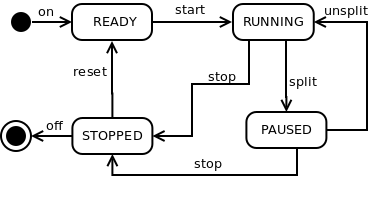
\includegraphics[scale=0.5]{figures/measurements_stopwatch}
\caption{Stopwatch FSM for testing}
\label{fig:measurements_stopwatch}
\end{figure}

\begin{table}[htb]
\begin{center}
\begin{tabular}{|l|}
\hline
	\textbf{Hardware specification}\\\hline
	\textbf{CPU}: 2.7GHz dual-core Intel Core i5 processor with 3MB shared L3 cache\\
	\textbf{RAM}: 8GB 1866MHz LPDDR3 RAM\\
	\textbf{Storage}: 128GB PCIe-based flash storage\\
\hline
\end{tabular}
\end{center}
\caption{\label{tab:hardwarespecification} Measurement architecture}
\end{table}

\begin{figure}[htp]
\centering
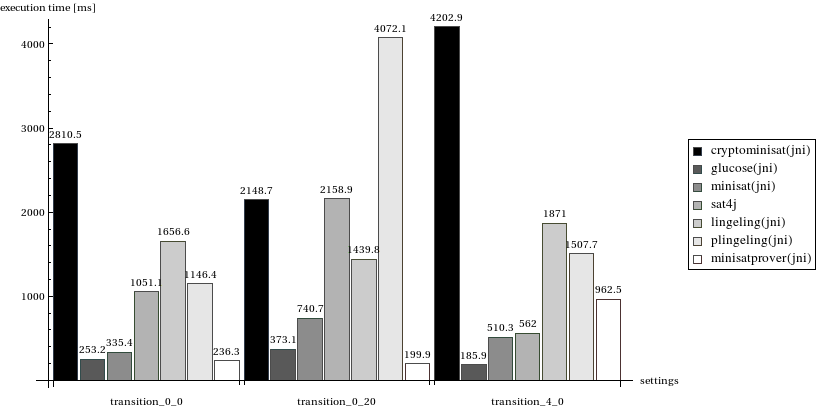
\includegraphics[scale=0.5]{figures/measurements_alloy_settings}
\caption{Adjusting Alloy settings}
\label{fig:measurements_alloy_settings}
\end{figure}

\begin{figure}[htp]
\centering
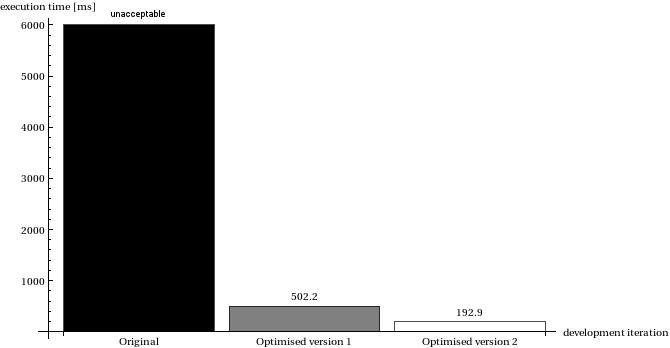
\includegraphics[scale=0.5]{figures/measurements_optimalizations}
\caption{Optimalisation results}
\label{fig:measurements_optimalizations}
\end{figure}

\begin{figure}[htp]
\centering
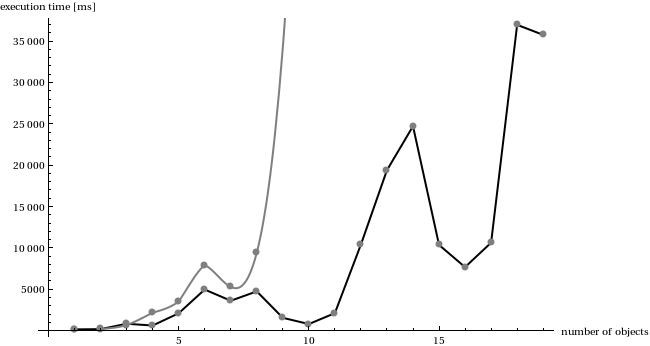
\includegraphics[scale=0.5]{figures/measurements_scalability}
\caption{Scalability results}
\label{fig:measurements_scalability}
\end{figure}

% chapter measurements (end)